\newcommand{\Seq}{C0}
\newcommand{\SeqClassParMeth}{C1}
\newcommand{\ParClassSeqMeth}{C2}
\newcommand{\ParClassParMeth}{C3}
\newcommand{\Fork}{F}
\newcommand{\ForkSeq}{\Fork{}\Seq{}}
\newcommand{\ForkParMeth}{\Fork{}\SeqClassParMeth{}}

\section{Parallel Execution of Test Suites}
\label{sec:modes}

\begin{figure}[t!]
  \centering
  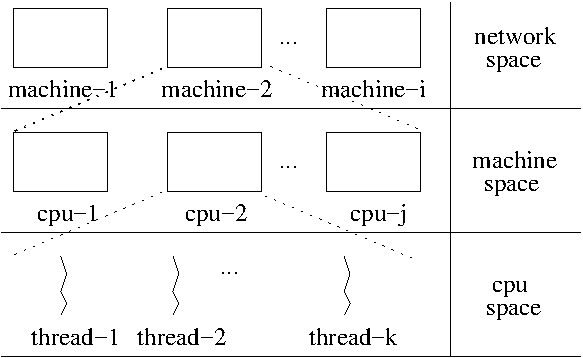
\includegraphics[width=0.35\textwidth]{figs/parallel-levels.pdf}
  \vspace{-1ex}
  \caption{\label{fig:levels}Levels of parallelism.}
\end{figure}

Parallelism in test execution can be obtained at different levels.
Figure~\ref{fig:levels} illustrates this.  The highest level indicates
parallelism that can be obtained through different machines on the
network.  For instance, using virtual machines from a cloud service to
distribute test execution.  The lowest levels denote parallelism
obtained within a single machine.  These levels are complementary:
low-level parallelization leverages the computing power of server
nodes whereas high-level schemes leverage the aggregate processing
power of the farm.

This paper focuses at low-level parallelism, where computation can be
offloaded at different CPUs within a machine and at different threads
within each CPU.  This form of parallelism is enabled through build
systems (spawning processes in different CPUs) and testing frameworks
(spawning threads in a CPU).  It is important to note that a variety
of testing frameworks provide today support for parallel test
execution (e.g., JUnit~\cite{junit-org}, TestNG~\cite{testng}, and
NUnit~\cite{nunit}) as to leverage the power of multi-core processors.
In the following, we elaborate relevant features of testing frameworks
and build systems.  We focused on Java, Maven, and JUnit but the
discussion can be generalized to other language and tools.

\subsection{Testing Frameworks}
\label{sec:frameworks}

The list below shows the choices to control parallelism within a Java
virtual machine (JVM) which runs in a single process of the CPU.

\begin{itemize}
\item
    \textbf{Sequential (\Seq).}~No parallelism is involved.
\item
    \textbf{Sequential classes; parallel methods
        (\SeqClassParMeth).}~This configuration corresponds to the
        sequential execution of test classes and test methods run in
        multiple threads.
\item
    \textbf{Parallel classes; sequential methods
        (\ParClassSeqMeth{}).}~This configuration corresponds to the
        execution of test classes in multiple threads and tests run
        sequentially within each thread.
\item
    \textbf{Parallel classes; Parallel methods
        (\ParClassParMeth).}~This configuration corresponds
        conceptually to the union of \ParClassSeqMeth{} and
        \SeqClassParMeth{}: the testing framework runs test methods
        from several classes on multiple threads.
\end{itemize}

The configuration \Seq{} is a proper fit for short-running test suites
since this is the default configuration and the execution provides
feedback in an acceptable time. However, for costly suites, it is
impractical for developers to wait long-running executions to take
action.  In this scenario, the remaining configuration may help to
amortize the execution cost depending on how the test suite was
designed. For instance, the configuration \SeqClassParMeth{} may
speedup the execution of test suites composed large test classes since
the cost of running all test methods is amortized by a pool of
threads. Similarly, the configuration \ParClassSeqMeth{} may speedup
test suites composed by several small test classes. Notice that both
configurations \ParClassSeqMeth{} and \SeqClassParMeth{} avoid
data-race condition at different levels. For instance, if two test methods performs operations in a same variable, the configuration \SeqClassParMeth{} would be preferable. Finally, 
the configuration \ParClassParMeth{} does not impose any sequential 
execution but it is more likely to manifest data-races as methods 
from different classes run in parallel.

\subsection{Build Systems}
\label{sec:builder}

The list below shows the choices to control parallelism through build
systems which uses multiple JVMs on different processes each:

\begin{itemize}
\item
    \textbf{Forked classes; sequential methods (\ForkSeq).}~This
        configuration corresponds to the parallel execution of test
        classes on different JVMs with test methods running
        sequentially within each JVM.
\item
    \textbf{Forked classes; parallel methods (\ForkParMeth).}~This
        configuration corresponds to the parallel execution of test
        classes on different JVMs with test methods running on
        multiple threads within each JVM.
\end{itemize}

Several build systems support the execution of test classes in forked
processes running a JVM. In the configuration \ForkSeq{}, each spawned
process runs a different test class at time and the builder merges the
results from each execution. In the configuration \ForkParMeth{}, the
build system forwards settings to the underlying testing framework to
enable parallel execution within each process in addition to running
test classes on different processes.  However, some configurations
(\eg, \ParClassSeqMeth) may not take effect since only one test class
can run in a forked process at time.  To the best of our knowledge, we
are unaware of any build system capable of running multiple classes at
time within a forked process.

\subsubsection*{Illustration}~Figure~\ref{fig:surefire} illustrates
the support of parallel execution with the configuration
\ForkParMeth{} on Maven, a popular build system in Java projects.
Maven uses a configuration file based on XML (known as \pomf{}) to
define tasks related to the project building and these tasks are
performed several plugins. \Jbc{falar do surefire e explicar a
configuracao ilustrada - Surefire levanta uma JVM por core e cria uma
pool de 5 threads em cada JVM para executar testes em paralelo.}

\begin{figure}[h!]
\centering
\scriptsize
\lstset{
    escapeinside={@}{@},
    numbers=left,xleftmargin=1em,frame=single,framexleftmargin=0.5em,
    basicstyle=\ttfamily\scriptsize, boxpos=c, numberstyle=\tiny,
    morekeywords={parallel, threadCount, perCoreThreadCount,
    forkCount, reuseFork},
    deletekeywords={true}
}
\begin{lstlisting}
<plugin>
    <groupId>org.apache.maven.plugins</groupId>
    <artifactId>maven-surefire-plugin</artifactId>
    <configuration>
        <forkCount>1C</forkCount>
        <parallel>methods</parallel>
        <threadCount>5</threadCount>
    </configuration>
</plugin>
\end{lstlisting}
    \caption{\label{fig:surefire} Maven setup with the configuration
    \ForkParMeth{}.  Maven forks one JVM per core (\CodeIn{forkCount}
    parameter) and uses five threads (\CodeIn{threadCount} parameter)
    to run methods (\CodeIn{parallel} parameter) within each JVM.}
\end{figure}

%%  LocalWords:  parallelization CPUs JUnit TestNG NUnit multi JVM de
%%  LocalWords:  JVMs falar explicar configuracao ilustrada levanta
%%  LocalWords:  uma por cria cada executar paralelo escapeinside
